%% fig_vandermonde.tex   (generated by make_round40.py; do not edit by hand)
%% Diagonal complete intersections of Vandermonde type (thm:vandermonde, cor:twodiagonal).
\documentclass[tikz,border=8pt]{standalone}
\usepackage{amsmath,amssymb}
\usetikzlibrary{arrows.meta,calc,decorations.pathreplacing}
%% palette.tex -- shared colour definitions for the figures
\definecolor{PInk}{RGB}{26,32,44}
\definecolor{PBlue}{RGB}{37,82,139}
\definecolor{PTeal}{RGB}{23,127,125}
\definecolor{POchre}{RGB}{193,138,44}
\definecolor{PClay}{RGB}{178,74,58}
\definecolor{PSlate}{RGB}{108,122,137}
\definecolor{PViolet}{RGB}{110,86,150}
\definecolor{WBlue}{RGB}{223,234,246}
\definecolor{WTeal}{RGB}{220,238,236}
\definecolor{WOchre}{RGB}{250,240,218}
\definecolor{WClay}{RGB}{247,229,224}
\definecolor{WSlate}{RGB}{238,241,244}
\definecolor{PMag}{RGB}{158,58,110}
\definecolor{PGrass}{RGB}{62,124,66}
\definecolor{PAmber}{RGB}{214,112,38}
\definecolor{PIndigo}{RGB}{58,64,140}
\definecolor{PRule}{RGB}{176,186,197}

%% shared macros so the standalone figures match the paper
\providecommand{\QQ}{\mathbb{Q}}
\providecommand{\ZZ}{\mathbb{Z}}
\providecommand{\RR}{\mathbb{R}}
\providecommand{\CC}{\mathbb{C}}
\providecommand{\PP}{\mathbb{P}}
\providecommand{\Kx}{K^{\times}}
\providecommand{\HW}{W}
\providecommand{\Nm}{\mathrm{N}}
\providecommand{\Hdg}{\mathrm{Hdg}}
\providecommand{\NS}{\mathrm{NS}}
\providecommand{\cA}{\mathcal{A}}
\providecommand{\cD}{\mathcal{D}}
\providecommand{\cF}{\mathcal{F}}
\providecommand{\cP}{\mathcal{P}}
\providecommand{\cO}{\mathcal{O}}
\providecommand{\cQ}{\mathcal{Q}}
\providecommand{\bbar}[1]{\overline{#1}}
\providecommand{\ch}{\operatorname{ch}}
\providecommand{\End}{\mathrm{End}}
\providecommand{\Ext}{\operatorname{Ext}}
\providecommand{\Supp}{\operatorname{Supp}}

\begin{document}
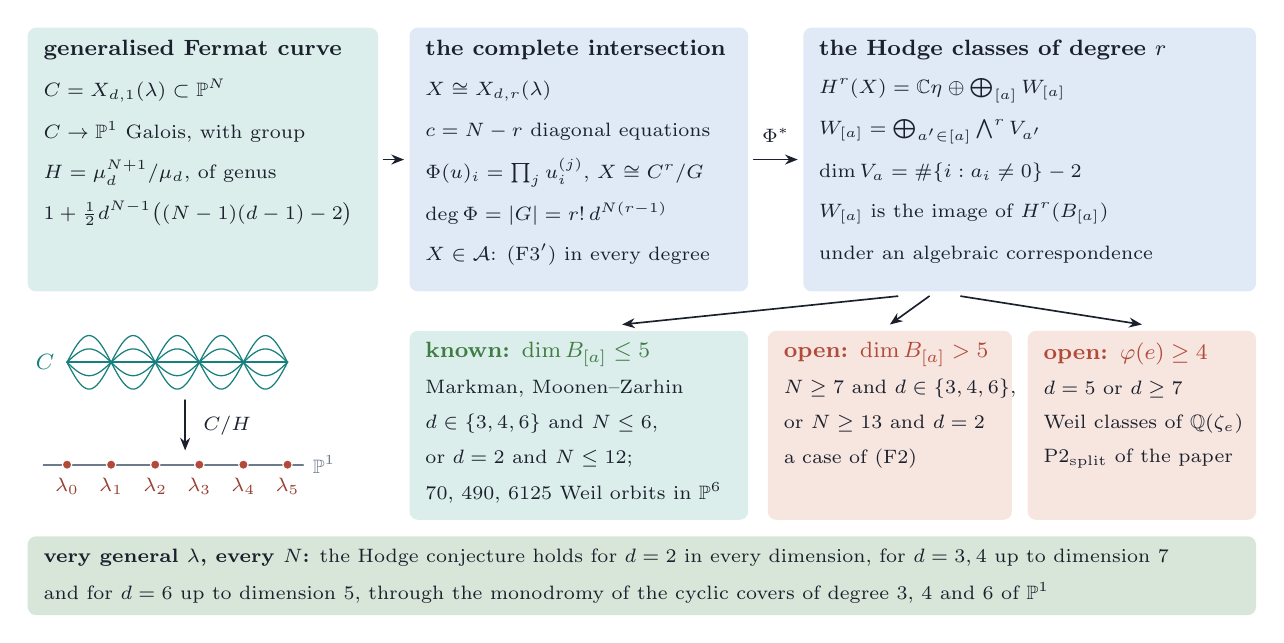
\begin{tikzpicture}[x=1cm,y=1cm,line join=round,line cap=round,
  font=\small,text=PInk,lbl/.style={inner sep=1pt}]
  \path[fill=WTeal,draw=none,rounded corners=3.0pt] (0.0500,2.9500) rectangle (4.5000,6.3000);
  \path[fill=WBlue,draw=none,rounded corners=3.0pt] (4.9000,2.9500) rectangle (9.2000,6.3000);
  \path[fill=WBlue,draw=none,rounded corners=3.0pt] (9.9000,2.9500) rectangle (15.6500,6.3000);
  \path[fill=WTeal,draw=none,rounded corners=3.0pt] (4.9000,0.0500) rectangle (9.2000,2.4500);
  \path[fill=WClay,draw=none,rounded corners=3.0pt] (9.4500,0.0500) rectangle (12.5500,2.4500);
  \path[fill=WClay,draw=none,rounded corners=3.0pt] (12.7500,0.0500) rectangle (15.6500,2.4500);
  \path[fill=PGrass!20!white,draw=none,rounded corners=3.0pt] (0.0500,-1.1600) rectangle (15.6500,-0.1600);
  \draw[PSlate,line width=0.6pt] (0.2500,0.7500) -- (3.5500,0.7500);
  \path[fill=PClay,draw=white,line width=0.40pt] (0.5500,0.7500) circle (1.70pt);
  \path[fill=PClay,draw=white,line width=0.40pt] (1.1100,0.7500) circle (1.70pt);
  \path[fill=PClay,draw=white,line width=0.40pt] (1.6700,0.7500) circle (1.70pt);
  \path[fill=PClay,draw=white,line width=0.40pt] (2.2300,0.7500) circle (1.70pt);
  \path[fill=PClay,draw=white,line width=0.40pt] (2.7900,0.7500) circle (1.70pt);
  \path[fill=PClay,draw=white,line width=0.40pt] (3.3500,0.7500) circle (1.70pt);
  \draw[PTeal,line width=0.45pt] (0.5500,2.0500) -- (0.5733,2.0056) -- (0.5967,1.9620) -- (0.6200,1.9199) -- (0.6433,1.8800) -- (0.6667,1.8430) -- (0.6900,1.8096) -- (0.7133,1.7803) -- (0.7367,1.7556) -- (0.7600,1.7359) -- (0.7833,1.7216) -- (0.8067,1.7129) -- (0.8300,1.7100) -- (0.8533,1.7129) -- (0.8767,1.7216) -- (0.9000,1.7359) -- (0.9233,1.7556) -- (0.9467,1.7803) -- (0.9700,1.8096) -- (0.9933,1.8430) -- (1.0167,1.8800) -- (1.0400,1.9199) -- (1.0633,1.9620) -- (1.0867,2.0056) -- (1.1100,2.0500) -- (1.1333,2.0056) -- (1.1567,1.9620) -- (1.1800,1.9199) -- (1.2033,1.8800) -- (1.2267,1.8430) -- (1.2500,1.8096) -- (1.2733,1.7803) -- (1.2967,1.7556) -- (1.3200,1.7359) -- (1.3433,1.7216) -- (1.3667,1.7129) -- (1.3900,1.7100) -- (1.4133,1.7129) -- (1.4367,1.7216) -- (1.4600,1.7359) -- (1.4833,1.7556) -- (1.5067,1.7803) -- (1.5300,1.8096) -- (1.5533,1.8430) -- (1.5767,1.8800) -- (1.6000,1.9199) -- (1.6233,1.9620) -- (1.6467,2.0056) -- (1.6700,2.0500) -- (1.6933,2.0056) -- (1.7167,1.9620) -- (1.7400,1.9199) -- (1.7633,1.8800) -- (1.7867,1.8430) -- (1.8100,1.8096) -- (1.8333,1.7803) -- (1.8567,1.7556) -- (1.8800,1.7359) -- (1.9033,1.7216) -- (1.9267,1.7129) -- (1.9500,1.7100) -- (1.9733,1.7129) -- (1.9967,1.7216) -- (2.0200,1.7359) -- (2.0433,1.7556) -- (2.0667,1.7803) -- (2.0900,1.8096) -- (2.1133,1.8430) -- (2.1367,1.8800) -- (2.1600,1.9199) -- (2.1833,1.9620) -- (2.2067,2.0056) -- (2.2300,2.0500) -- (2.2533,2.0056) -- (2.2767,1.9620) -- (2.3000,1.9199) -- (2.3233,1.8800) -- (2.3467,1.8430) -- (2.3700,1.8096) -- (2.3933,1.7803) -- (2.4167,1.7556) -- (2.4400,1.7359) -- (2.4633,1.7216) -- (2.4867,1.7129) -- (2.5100,1.7100) -- (2.5333,1.7129) -- (2.5567,1.7216) -- (2.5800,1.7359) -- (2.6033,1.7556) -- (2.6267,1.7803) -- (2.6500,1.8096) -- (2.6733,1.8430) -- (2.6967,1.8800) -- (2.7200,1.9199) -- (2.7433,1.9620) -- (2.7667,2.0056) -- (2.7900,2.0500) -- (2.8133,2.0056) -- (2.8367,1.9620) -- (2.8600,1.9199) -- (2.8833,1.8800) -- (2.9067,1.8430) -- (2.9300,1.8096) -- (2.9533,1.7803) -- (2.9767,1.7556) -- (3.0000,1.7359) -- (3.0233,1.7216) -- (3.0467,1.7129) -- (3.0700,1.7100) -- (3.0933,1.7129) -- (3.1167,1.7216) -- (3.1400,1.7359) -- (3.1633,1.7556) -- (3.1867,1.7803) -- (3.2100,1.8096) -- (3.2333,1.8430) -- (3.2567,1.8800) -- (3.2800,1.9199) -- (3.3033,1.9620) -- (3.3267,2.0056) -- (3.3500,2.0500);
  \draw[PTeal,line width=0.45pt] (0.5500,2.0500) -- (0.5733,2.0278) -- (0.5967,2.0060) -- (0.6200,1.9849) -- (0.6433,1.9650) -- (0.6667,1.9465) -- (0.6900,1.9298) -- (0.7133,1.9151) -- (0.7367,1.9028) -- (0.7600,1.8929) -- (0.7833,1.8858) -- (0.8067,1.8815) -- (0.8300,1.8800) -- (0.8533,1.8815) -- (0.8767,1.8858) -- (0.9000,1.8929) -- (0.9233,1.9028) -- (0.9467,1.9151) -- (0.9700,1.9298) -- (0.9933,1.9465) -- (1.0167,1.9650) -- (1.0400,1.9849) -- (1.0633,2.0060) -- (1.0867,2.0278) -- (1.1100,2.0500) -- (1.1333,2.0278) -- (1.1567,2.0060) -- (1.1800,1.9849) -- (1.2033,1.9650) -- (1.2267,1.9465) -- (1.2500,1.9298) -- (1.2733,1.9151) -- (1.2967,1.9028) -- (1.3200,1.8929) -- (1.3433,1.8858) -- (1.3667,1.8815) -- (1.3900,1.8800) -- (1.4133,1.8815) -- (1.4367,1.8858) -- (1.4600,1.8929) -- (1.4833,1.9028) -- (1.5067,1.9151) -- (1.5300,1.9298) -- (1.5533,1.9465) -- (1.5767,1.9650) -- (1.6000,1.9849) -- (1.6233,2.0060) -- (1.6467,2.0278) -- (1.6700,2.0500) -- (1.6933,2.0278) -- (1.7167,2.0060) -- (1.7400,1.9849) -- (1.7633,1.9650) -- (1.7867,1.9465) -- (1.8100,1.9298) -- (1.8333,1.9151) -- (1.8567,1.9028) -- (1.8800,1.8929) -- (1.9033,1.8858) -- (1.9267,1.8815) -- (1.9500,1.8800) -- (1.9733,1.8815) -- (1.9967,1.8858) -- (2.0200,1.8929) -- (2.0433,1.9028) -- (2.0667,1.9151) -- (2.0900,1.9298) -- (2.1133,1.9465) -- (2.1367,1.9650) -- (2.1600,1.9849) -- (2.1833,2.0060) -- (2.2067,2.0278) -- (2.2300,2.0500) -- (2.2533,2.0278) -- (2.2767,2.0060) -- (2.3000,1.9849) -- (2.3233,1.9650) -- (2.3467,1.9465) -- (2.3700,1.9298) -- (2.3933,1.9151) -- (2.4167,1.9028) -- (2.4400,1.8929) -- (2.4633,1.8858) -- (2.4867,1.8815) -- (2.5100,1.8800) -- (2.5333,1.8815) -- (2.5567,1.8858) -- (2.5800,1.8929) -- (2.6033,1.9028) -- (2.6267,1.9151) -- (2.6500,1.9298) -- (2.6733,1.9465) -- (2.6967,1.9650) -- (2.7200,1.9849) -- (2.7433,2.0060) -- (2.7667,2.0278) -- (2.7900,2.0500) -- (2.8133,2.0278) -- (2.8367,2.0060) -- (2.8600,1.9849) -- (2.8833,1.9650) -- (2.9067,1.9465) -- (2.9300,1.9298) -- (2.9533,1.9151) -- (2.9767,1.9028) -- (3.0000,1.8929) -- (3.0233,1.8858) -- (3.0467,1.8815) -- (3.0700,1.8800) -- (3.0933,1.8815) -- (3.1167,1.8858) -- (3.1400,1.8929) -- (3.1633,1.9028) -- (3.1867,1.9151) -- (3.2100,1.9298) -- (3.2333,1.9465) -- (3.2567,1.9650) -- (3.2800,1.9849) -- (3.3033,2.0060) -- (3.3267,2.0278) -- (3.3500,2.0500);
  \draw[PTeal,line width=0.75pt] (0.5500,2.0500) -- (0.5733,2.0500) -- (0.5967,2.0500) -- (0.6200,2.0500) -- (0.6433,2.0500) -- (0.6667,2.0500) -- (0.6900,2.0500) -- (0.7133,2.0500) -- (0.7367,2.0500) -- (0.7600,2.0500) -- (0.7833,2.0500) -- (0.8067,2.0500) -- (0.8300,2.0500) -- (0.8533,2.0500) -- (0.8767,2.0500) -- (0.9000,2.0500) -- (0.9233,2.0500) -- (0.9467,2.0500) -- (0.9700,2.0500) -- (0.9933,2.0500) -- (1.0167,2.0500) -- (1.0400,2.0500) -- (1.0633,2.0500) -- (1.0867,2.0500) -- (1.1100,2.0500) -- (1.1333,2.0500) -- (1.1567,2.0500) -- (1.1800,2.0500) -- (1.2033,2.0500) -- (1.2267,2.0500) -- (1.2500,2.0500) -- (1.2733,2.0500) -- (1.2967,2.0500) -- (1.3200,2.0500) -- (1.3433,2.0500) -- (1.3667,2.0500) -- (1.3900,2.0500) -- (1.4133,2.0500) -- (1.4367,2.0500) -- (1.4600,2.0500) -- (1.4833,2.0500) -- (1.5067,2.0500) -- (1.5300,2.0500) -- (1.5533,2.0500) -- (1.5767,2.0500) -- (1.6000,2.0500) -- (1.6233,2.0500) -- (1.6467,2.0500) -- (1.6700,2.0500) -- (1.6933,2.0500) -- (1.7167,2.0500) -- (1.7400,2.0500) -- (1.7633,2.0500) -- (1.7867,2.0500) -- (1.8100,2.0500) -- (1.8333,2.0500) -- (1.8567,2.0500) -- (1.8800,2.0500) -- (1.9033,2.0500) -- (1.9267,2.0500) -- (1.9500,2.0500) -- (1.9733,2.0500) -- (1.9967,2.0500) -- (2.0200,2.0500) -- (2.0433,2.0500) -- (2.0667,2.0500) -- (2.0900,2.0500) -- (2.1133,2.0500) -- (2.1367,2.0500) -- (2.1600,2.0500) -- (2.1833,2.0500) -- (2.2067,2.0500) -- (2.2300,2.0500) -- (2.2533,2.0500) -- (2.2767,2.0500) -- (2.3000,2.0500) -- (2.3233,2.0500) -- (2.3467,2.0500) -- (2.3700,2.0500) -- (2.3933,2.0500) -- (2.4167,2.0500) -- (2.4400,2.0500) -- (2.4633,2.0500) -- (2.4867,2.0500) -- (2.5100,2.0500) -- (2.5333,2.0500) -- (2.5567,2.0500) -- (2.5800,2.0500) -- (2.6033,2.0500) -- (2.6267,2.0500) -- (2.6500,2.0500) -- (2.6733,2.0500) -- (2.6967,2.0500) -- (2.7200,2.0500) -- (2.7433,2.0500) -- (2.7667,2.0500) -- (2.7900,2.0500) -- (2.8133,2.0500) -- (2.8367,2.0500) -- (2.8600,2.0500) -- (2.8833,2.0500) -- (2.9067,2.0500) -- (2.9300,2.0500) -- (2.9533,2.0500) -- (2.9767,2.0500) -- (3.0000,2.0500) -- (3.0233,2.0500) -- (3.0467,2.0500) -- (3.0700,2.0500) -- (3.0933,2.0500) -- (3.1167,2.0500) -- (3.1400,2.0500) -- (3.1633,2.0500) -- (3.1867,2.0500) -- (3.2100,2.0500) -- (3.2333,2.0500) -- (3.2567,2.0500) -- (3.2800,2.0500) -- (3.3033,2.0500) -- (3.3267,2.0500) -- (3.3500,2.0500);
  \draw[PTeal,line width=0.45pt] (0.5500,2.0500) -- (0.5733,2.0722) -- (0.5967,2.0940) -- (0.6200,2.1151) -- (0.6433,2.1350) -- (0.6667,2.1535) -- (0.6900,2.1702) -- (0.7133,2.1849) -- (0.7367,2.1972) -- (0.7600,2.2071) -- (0.7833,2.2142) -- (0.8067,2.2185) -- (0.8300,2.2200) -- (0.8533,2.2185) -- (0.8767,2.2142) -- (0.9000,2.2071) -- (0.9233,2.1972) -- (0.9467,2.1849) -- (0.9700,2.1702) -- (0.9933,2.1535) -- (1.0167,2.1350) -- (1.0400,2.1151) -- (1.0633,2.0940) -- (1.0867,2.0722) -- (1.1100,2.0500) -- (1.1333,2.0722) -- (1.1567,2.0940) -- (1.1800,2.1151) -- (1.2033,2.1350) -- (1.2267,2.1535) -- (1.2500,2.1702) -- (1.2733,2.1849) -- (1.2967,2.1972) -- (1.3200,2.2071) -- (1.3433,2.2142) -- (1.3667,2.2185) -- (1.3900,2.2200) -- (1.4133,2.2185) -- (1.4367,2.2142) -- (1.4600,2.2071) -- (1.4833,2.1972) -- (1.5067,2.1849) -- (1.5300,2.1702) -- (1.5533,2.1535) -- (1.5767,2.1350) -- (1.6000,2.1151) -- (1.6233,2.0940) -- (1.6467,2.0722) -- (1.6700,2.0500) -- (1.6933,2.0722) -- (1.7167,2.0940) -- (1.7400,2.1151) -- (1.7633,2.1350) -- (1.7867,2.1535) -- (1.8100,2.1702) -- (1.8333,2.1849) -- (1.8567,2.1972) -- (1.8800,2.2071) -- (1.9033,2.2142) -- (1.9267,2.2185) -- (1.9500,2.2200) -- (1.9733,2.2185) -- (1.9967,2.2142) -- (2.0200,2.2071) -- (2.0433,2.1972) -- (2.0667,2.1849) -- (2.0900,2.1702) -- (2.1133,2.1535) -- (2.1367,2.1350) -- (2.1600,2.1151) -- (2.1833,2.0940) -- (2.2067,2.0722) -- (2.2300,2.0500) -- (2.2533,2.0722) -- (2.2767,2.0940) -- (2.3000,2.1151) -- (2.3233,2.1350) -- (2.3467,2.1535) -- (2.3700,2.1702) -- (2.3933,2.1849) -- (2.4167,2.1972) -- (2.4400,2.2071) -- (2.4633,2.2142) -- (2.4867,2.2185) -- (2.5100,2.2200) -- (2.5333,2.2185) -- (2.5567,2.2142) -- (2.5800,2.2071) -- (2.6033,2.1972) -- (2.6267,2.1849) -- (2.6500,2.1702) -- (2.6733,2.1535) -- (2.6967,2.1350) -- (2.7200,2.1151) -- (2.7433,2.0940) -- (2.7667,2.0722) -- (2.7900,2.0500) -- (2.8133,2.0722) -- (2.8367,2.0940) -- (2.8600,2.1151) -- (2.8833,2.1350) -- (2.9067,2.1535) -- (2.9300,2.1702) -- (2.9533,2.1849) -- (2.9767,2.1972) -- (3.0000,2.2071) -- (3.0233,2.2142) -- (3.0467,2.2185) -- (3.0700,2.2200) -- (3.0933,2.2185) -- (3.1167,2.2142) -- (3.1400,2.2071) -- (3.1633,2.1972) -- (3.1867,2.1849) -- (3.2100,2.1702) -- (3.2333,2.1535) -- (3.2567,2.1350) -- (3.2800,2.1151) -- (3.3033,2.0940) -- (3.3267,2.0722) -- (3.3500,2.0500);
  \draw[PTeal,line width=0.45pt] (0.5500,2.0500) -- (0.5733,2.0944) -- (0.5967,2.1380) -- (0.6200,2.1801) -- (0.6433,2.2200) -- (0.6667,2.2570) -- (0.6900,2.2904) -- (0.7133,2.3197) -- (0.7367,2.3444) -- (0.7600,2.3641) -- (0.7833,2.3784) -- (0.8067,2.3871) -- (0.8300,2.3900) -- (0.8533,2.3871) -- (0.8767,2.3784) -- (0.9000,2.3641) -- (0.9233,2.3444) -- (0.9467,2.3197) -- (0.9700,2.2904) -- (0.9933,2.2570) -- (1.0167,2.2200) -- (1.0400,2.1801) -- (1.0633,2.1380) -- (1.0867,2.0944) -- (1.1100,2.0500) -- (1.1333,2.0944) -- (1.1567,2.1380) -- (1.1800,2.1801) -- (1.2033,2.2200) -- (1.2267,2.2570) -- (1.2500,2.2904) -- (1.2733,2.3197) -- (1.2967,2.3444) -- (1.3200,2.3641) -- (1.3433,2.3784) -- (1.3667,2.3871) -- (1.3900,2.3900) -- (1.4133,2.3871) -- (1.4367,2.3784) -- (1.4600,2.3641) -- (1.4833,2.3444) -- (1.5067,2.3197) -- (1.5300,2.2904) -- (1.5533,2.2570) -- (1.5767,2.2200) -- (1.6000,2.1801) -- (1.6233,2.1380) -- (1.6467,2.0944) -- (1.6700,2.0500) -- (1.6933,2.0944) -- (1.7167,2.1380) -- (1.7400,2.1801) -- (1.7633,2.2200) -- (1.7867,2.2570) -- (1.8100,2.2904) -- (1.8333,2.3197) -- (1.8567,2.3444) -- (1.8800,2.3641) -- (1.9033,2.3784) -- (1.9267,2.3871) -- (1.9500,2.3900) -- (1.9733,2.3871) -- (1.9967,2.3784) -- (2.0200,2.3641) -- (2.0433,2.3444) -- (2.0667,2.3197) -- (2.0900,2.2904) -- (2.1133,2.2570) -- (2.1367,2.2200) -- (2.1600,2.1801) -- (2.1833,2.1380) -- (2.2067,2.0944) -- (2.2300,2.0500) -- (2.2533,2.0944) -- (2.2767,2.1380) -- (2.3000,2.1801) -- (2.3233,2.2200) -- (2.3467,2.2570) -- (2.3700,2.2904) -- (2.3933,2.3197) -- (2.4167,2.3444) -- (2.4400,2.3641) -- (2.4633,2.3784) -- (2.4867,2.3871) -- (2.5100,2.3900) -- (2.5333,2.3871) -- (2.5567,2.3784) -- (2.5800,2.3641) -- (2.6033,2.3444) -- (2.6267,2.3197) -- (2.6500,2.2904) -- (2.6733,2.2570) -- (2.6967,2.2200) -- (2.7200,2.1801) -- (2.7433,2.1380) -- (2.7667,2.0944) -- (2.7900,2.0500) -- (2.8133,2.0944) -- (2.8367,2.1380) -- (2.8600,2.1801) -- (2.8833,2.2200) -- (2.9067,2.2570) -- (2.9300,2.2904) -- (2.9533,2.3197) -- (2.9767,2.3444) -- (3.0000,2.3641) -- (3.0233,2.3784) -- (3.0467,2.3871) -- (3.0700,2.3900) -- (3.0933,2.3871) -- (3.1167,2.3784) -- (3.1400,2.3641) -- (3.1633,2.3444) -- (3.1867,2.3197) -- (3.2100,2.2904) -- (3.2333,2.2570) -- (3.2567,2.2200) -- (3.2800,2.1801) -- (3.3033,2.1380) -- (3.3267,2.0944) -- (3.3500,2.0500);
  \draw[PInk,line width=0.6pt,-{Stealth[length=4.6pt,width=3.6pt]}] (2.0500,1.5700) -- (2.0500,0.9300);
  \draw[PInk,line width=0.6pt,-{Stealth[length=4.6pt,width=3.6pt]}] (4.5700,4.6250) -- (4.8300,4.6250);
  \draw[PInk,line width=0.6pt,-{Stealth[length=4.6pt,width=3.6pt]}] (9.2700,4.6250) -- (9.8300,4.6250);
  \draw[PInk,line width=0.6pt,-{Stealth[length=4.6pt,width=3.6pt]}] (11.1000,2.8900) -- (7.6000,2.5300);
  \draw[PInk,line width=0.6pt,-{Stealth[length=4.6pt,width=3.6pt]}] (11.5000,2.8900) -- (11.0000,2.5300);
  \draw[PInk,line width=0.6pt,-{Stealth[length=4.6pt,width=3.6pt]}] (11.9000,2.8900) -- (14.2000,2.5300);
  \node[lbl,anchor=north,text=PClay!85!black,font=\scriptsize] at (0.5500,0.6200) {$\lambda_{0}$};
  \node[lbl,anchor=north,text=PClay!85!black,font=\scriptsize] at (1.1100,0.6200) {$\lambda_{1}$};
  \node[lbl,anchor=north,text=PClay!85!black,font=\scriptsize] at (1.6700,0.6200) {$\lambda_{2}$};
  \node[lbl,anchor=north,text=PClay!85!black,font=\scriptsize] at (2.2300,0.6200) {$\lambda_{3}$};
  \node[lbl,anchor=north,text=PClay!85!black,font=\scriptsize] at (2.7900,0.6200) {$\lambda_{4}$};
  \node[lbl,anchor=north,text=PClay!85!black,font=\scriptsize] at (3.3500,0.6200) {$\lambda_{5}$};
  \node[lbl,anchor=west,text=PSlate,font=\scriptsize] at (3.6300,0.7500) {$\PP^{1}$};
  \node[lbl,anchor=east,text=PTeal,font=\footnotesize] at (0.4300,2.0500) {$C$};
  \node[lbl,anchor=west,text=PInk,font=\scriptsize] at (2.2400,1.2500) {$C/H$};
  \node[lbl,anchor=west,text=PInk,font=\footnotesize] at (0.2100,6.0200) {\textbf{generalised Fermat curve}};
  \node[lbl,anchor=west,text=PInk,font=\scriptsize] at (0.2100,5.5000) {$C=X_{d,1}(\lambda)\subset\PP^{N}$};
  \node[lbl,anchor=west,text=PInk,font=\scriptsize] at (0.2100,4.9800) {$C\to\PP^{1}$ Galois, with group};
  \node[lbl,anchor=west,text=PInk,font=\scriptsize] at (0.2100,4.4600) {$H=\mu_{d}^{N+1}/\mu_{d}$, of genus};
  \node[lbl,anchor=west,text=PInk,font=\scriptsize] at (0.2100,3.9400) {$1+\frac12d^{N-1}\bigl((N-1)(d-1)-2\bigr)$};
  \node[lbl,anchor=west,text=PInk,font=\footnotesize] at (5.0600,6.0200) {\textbf{the complete intersection}};
  \node[lbl,anchor=west,text=PInk,font=\scriptsize] at (5.0600,5.5000) {$X\cong X_{d,r}(\lambda)$};
  \node[lbl,anchor=west,text=PInk,font=\scriptsize] at (5.0600,4.9800) {$c=N-r$ diagonal equations};
  \node[lbl,anchor=west,text=PInk,font=\scriptsize] at (5.0600,4.4600) {$\Phi(u)_{i}=\prod_{j}u^{(j)}_{i}$, $X\cong C^{r}/G$};
  \node[lbl,anchor=west,text=PInk,font=\scriptsize] at (5.0600,3.9400) {$\deg\Phi=|G|=r!\,d^{N(r-1)}$};
  \node[lbl,anchor=west,text=PInk,font=\scriptsize] at (5.0600,3.4200) {$X\in\cA$: (F3$'$) in every degree};
  \node[lbl,anchor=west,text=PInk,font=\footnotesize] at (10.0600,6.0200) {\textbf{the Hodge classes of degree $r$}};
  \node[lbl,anchor=west,text=PInk,font=\scriptsize] at (10.0600,5.5000) {$H^{r}(X)=\CC\eta\oplus\bigoplus_{[a]}W_{[a]}$};
  \node[lbl,anchor=west,text=PInk,font=\scriptsize] at (10.0600,4.9800) {$W_{[a]}=\bigoplus_{a'\in[a]}\bigwedge^{r}V_{a'}$};
  \node[lbl,anchor=west,text=PInk,font=\scriptsize] at (10.0600,4.4600) {$\dim V_{a}=\#\{i:a_{i}\ne0\}-2$};
  \node[lbl,anchor=west,text=PInk,font=\scriptsize] at (10.0600,3.9400) {$W_{[a]}$ is the image of $H^{r}(B_{[a]})$};
  \node[lbl,anchor=west,text=PInk,font=\scriptsize] at (10.0600,3.4200) {under an algebraic correspondence};
  \node[lbl,anchor=south,text=PInk,font=\scriptsize] at (9.5500,4.7950) {$\Phi^{*}$};
  \node[lbl,anchor=west,text=PGrass,font=\footnotesize] at (5.0600,2.1500) {\textbf{known: $\dim B_{[a]}\le5$}};
  \node[lbl,anchor=west,text=PInk,font=\scriptsize] at (5.0600,1.7100) {Markman, Moonen--Zarhin};
  \node[lbl,anchor=west,text=PInk,font=\scriptsize] at (5.0600,1.2700) {$d\in\{3,4,6\}$ and $N\le6$,};
  \node[lbl,anchor=west,text=PInk,font=\scriptsize] at (5.0600,0.8300) {or $d=2$ and $N\le12$;};
  \node[lbl,anchor=west,text=PInk,font=\scriptsize] at (5.0600,0.3900) {$70$, $490$, $6125$ Weil orbits in $\PP^{6}$};
  \node[lbl,anchor=west,text=PClay,font=\footnotesize] at (9.6100,2.1500) {\textbf{open: $\dim B_{[a]}>5$}};
  \node[lbl,anchor=west,text=PInk,font=\scriptsize] at (9.6100,1.7100) {$N\ge7$ and $d\in\{3,4,6\}$,};
  \node[lbl,anchor=west,text=PInk,font=\scriptsize] at (9.6100,1.2700) {or $N\ge13$ and $d=2$};
  \node[lbl,anchor=west,text=PInk,font=\scriptsize] at (9.6100,0.8300) {a case of (F2)};
  \node[lbl,anchor=west,text=PClay,font=\footnotesize] at (12.9100,2.1500) {\textbf{open: $\varphi(e)\ge4$}};
  \node[lbl,anchor=west,text=PInk,font=\scriptsize] at (12.9100,1.7100) {$d=5$ or $d\ge7$};
  \node[lbl,anchor=west,text=PInk,font=\scriptsize] at (12.9100,1.2700) {Weil classes of $\QQ(\zeta_{e})$};
  \node[lbl,anchor=west,text=PInk,font=\scriptsize] at (12.9100,0.8300) {$\mathrm{P2}_{\mathrm{split}}$ of the paper};
  \node[lbl,anchor=west,text=PInk,font=\scriptsize] at (0.2100,-0.4300) {\textbf{very general $\lambda$, every $N$:} the Hodge conjecture holds for $d=2$ in every dimension, for $d=3,4$ up to dimension $7$};
  \node[lbl,anchor=west,text=PInk,font=\scriptsize] at (0.2100,-0.8800) {and for $d=6$ up to dimension $5$, through the monodromy of the cyclic covers of degree $3$, $4$ and $6$ of $\PP^{1}$};
\end{tikzpicture}
\end{document}
